\documentclass{article}
\usepackage{icmcsmc2014}
\usepackage{times}
\usepackage{ifpdf}
\usepackage[english]{babel}
%\usepackage{cite}
\usepackage{fancyvrb}
\usepackage[autostyle]{csquotes}  
%%%%%%%%%%%%%%%%%%%%%%%% Some useful packages %%%%%%%%%%%%%%%%%%%%%%%%%%%%%%%
%%%%%%%%%%%%%%%%%%%%%%%% See related documentation %%%%%%%%%%%%%%%%%%%%%%%%%%
%\usepackage{amsmath} % popular packages from Am. Math. Soc. Please use the 
%\usepackage{amssymb} % related math environments (split, subequation, cases,
%\usepackage{amsfonts}% multline, etc.)
%\usepackage{bm}      % Bold Math package, defines the command \bf{}
%\usepackage{paralist}% extended list environments
%%subfig.sty is the modern replacement for subfigure.sty. However, subfig.sty 
%%requires and automatically loads caption.sty which overrides class handling 
%%of captions. To prevent this problem, preload caption.sty with caption=false 
%\usepackage[caption=false]{caption}
%\usepackage[font=footnotesize]{subfig}


%user defined variables
\def\papertitle{Advances in Modality}
\def\firstauthor{First author}
\def\secondauthor{Second author}
\def\thirdauthor{Third author}


% authors so far:
% AdC, Till, Jeff, Miguel

% adds the automatic
% Saves a lot of ouptut space in PDF... after conversion with the distiller
% Delete if you cannot get PS fonts working on your system.

% pdf-tex settings: detect automatically if run by latex or pdflatex
\newif\ifpdf
\ifx\pdfoutput\relax
\else
   \ifcase\pdfoutput
      \pdffalse
   \else
      \pdftrue
\fi

\ifpdf % compiling with pdflatex
  \usepackage[pdftex,
    pdftitle={\papertitle},
    pdfauthor={\firstauthor, \secondauthor, \thirdauthor},
    bookmarksnumbered, % use section numbers with bookmarks
    pdfstartview=XYZ % start with zoom=100% instead of full screen; 
                     % especially useful if working with a big screen :-)
   ]{hyperref}
  %\pdfcompresslevel=9

  \usepackage[pdftex]{graphicx}
  % declare the path(s) where your graphic files are and their extensions so 
  %you won't have to specify these with every instance of \includegraphics
  \graphicspath{{./figures/}}
  \DeclareGraphicsExtensions{.pdf,.jpeg,.png}

  \usepackage[figure,table]{hypcap}
\fi

%setup the hyperref package - make the links black without a surrounding frame
\hypersetup{
    colorlinks,%
    citecolor=black,%
    filecolor=black,%
    linkcolor=black,%
    urlcolor=black
}


% Title.
% ------
\title{\papertitle}

% Authors
% Please note that submissions are NOT anonymous, therefore 
% authors' names have to be VISIBLE in your manuscript. 
%
% Single address
% To use with only one author or several with the same address
% ---------------
%\oneauthor
%   {\firstauthor} {Affiliation1 \\ %
%     {\tt \href{mailto:author1@smcnetwork.org}{author1@smcnetwork.org}}}

%Two addresses
%--------------
% \twoauthors
%   {\firstauthor} {Affiliation1 \\ %
%     {\tt \href{mailto:author1@smcnetwork.org}{author1@smcnetwork.org}}}
%   {\secondauthor} {Affiliation2 \\ %
%     {\tt \href{mailto:author2@smcnetwork.org}{author2@smcnetwork.org}}}

% Three addresses
% --------------
 \threeauthors
   {\firstauthor} {Affiliation1 \\ %
     {\tt \href{mailto:author1@smcnetwork.org}{author1@smcnetwork.org}}}
   {\secondauthor} {Affiliation2 \\ %
     {\tt \href{mailto:author2@smcnetwork.org}{author2@smcnetwork.org}}}
   {\thirdauthor} { Affiliation3 \\ %
     {\tt \href{mailto:author3@smcnetwork.org}{author3@smcnetwork.org}}}

\newcommand{\todo}[1] {\emph{\textbf{TODO:} #1}}
\DefineShortVerb{\|}


% ***************************************** tA document starts here ***************
\begin{document}
%
\capstartfalse
\maketitle
\capstarttrue
%
\begin{abstract}
The Modality toolkit aims to improve and facilitate the use of digital technology within interactive sound art and music. 
Written in SuperCollider, it simplifies the creation of individual electronic instruments by combining custom sound engines with off-the-shelf controllers. 
To this end, a common code interface, |MKtl|, is used to connect controllers from various sources and protocols. 
Currently, HID and MIDI are supported; GUI-based interfaces can be created on the fly from interface descriptions.
\end{abstract}

\begin{figure}[h]
	\centering
		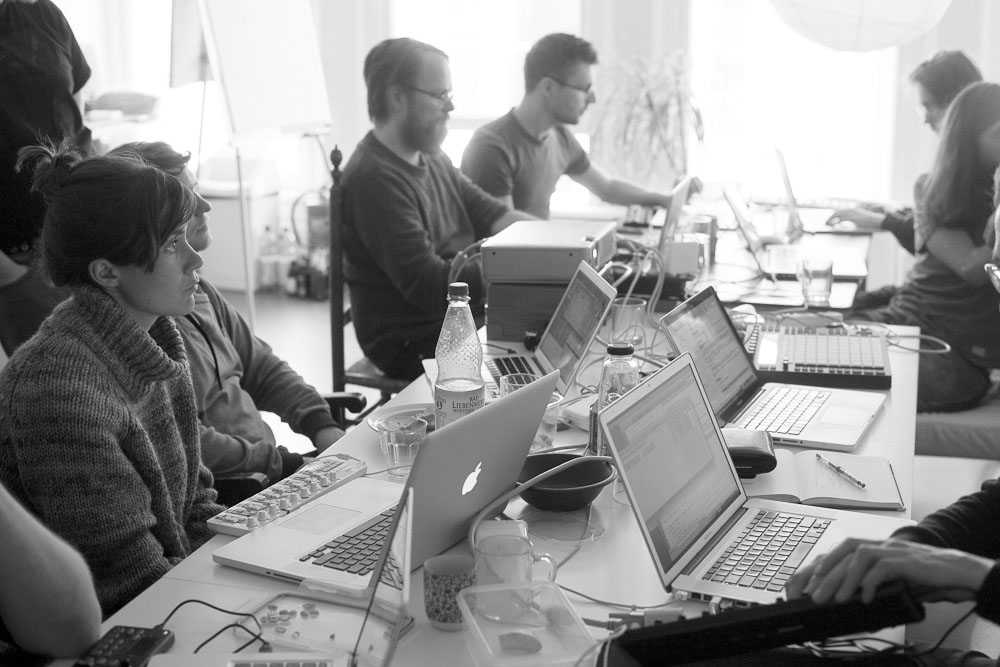
\includegraphics[width=.9\columnwidth]{../media/20140331-IMG_5976.jpg}
	\caption{Meeting 2014 in Amsterdam}
	\label{fig:media_20140331-IMG_5976}
\end{figure}

\section{Scope and Overview}
\label{sec:overview_of_modality_concept_and_aims}

The Modality project is dedicated to modal interaction with synthesis processes for physical control in performance. 
Its primary product is the Modality Toolkit, a library to facilitate straightforward access to hardware controllers in the SuperCollider programming language. 
It is designed and developed by the ModalityTeam, a group of people that see themselves as both users and developers, both of and for SuperCollider.

The name Modality arose from the idea to scaffold the creation of modal interfaces, i.e., to create interfaces where e.g., one physical controller can be used for different purposes or it is possible to switch its functionality, even at runtime. 
We belief that integration of such on-the-fly remapping features helps to create instruments that are flexible, powerful, and interesting to play. 
The strength of such a modal interface is that it allows for fast changes and more opportunity for sonic discovery as can be necessary when, for example, improvising with musicians playing acoustic instruments. 


\section{Towards modal control}
\label{sec:modal_control}

\emph{Tells about the scope of the modality group, how it was established and how the meetings work. Should especially include a description of the combination of developer meeting, public workshop and concert.}



\subsection{The modality way}
\label{sub:the_modality_way}

\emph{Tells about how the Modality meetings work, i.e., a description of the combination of developer meeting, public workshop and concerts.}


Over the last years, the ModalityTeam met four times at different places:

\begin{description}
	\item[October 2010, BEK, Bergen] Initiated by Jeff Carey and Bj\o{}rnar Habbestad, several experts and sound artists met to discuss about modal control in performance and rehearsal situations.
	Soon it became apparent that, for all attendees, easy access and outlining of modal control structures is of great interest. First sketches for uniform access were made based on the then already existing JITMIDIKtl extension, creating a more uniform access to controllers in the Ktl extension.
	
% 	\todo{add further description on founding meeting. Should do someone who actually was there.}
	
	\item[May 2011, STEIM, Amsterdam] Initial discussions unveiled the necessity for users to abstract from hardware dependencies and being able to do flexible routings and filtering incoming data.

	We therefore developed a new extension (a so-called Quark) for the in SuperCollider language that (partly) implemented two sets of functionalities:
	
	\begin{itemize}
		\item 	It was possible to query connected MIDI and HID hardware devices with an |MKtl| object. 
		Capabilities of each device were stored in a configuration file. 
		Rather than assigning functions via hardware-specific code (e.g. a MIDI control number, or an HID device element cookie), we thought of controllers as a combination of \emph{controller elements}, |MKtlElements|. 
		It was possible to associate a human-readable name with element-specific data.
		With the goal for future support of the serial port, OpenSoundControl, and other hardware interfaces, the workflow was designed as generic as needed to abstract from the actual backend.
		\item In addition, we worked on the |MDispatch| class, which allowed to create \emph{calculation units}; abstract filters that render output from a given input, like the conversion of a button press (two states: on/off) to one trigger event (on), or the calculation of slider speed. 
		Templates for commonly used functionality were created.
	\end{itemize}
	
	A stumbleblock at this point was that the HID implementation in SuperCollider on OSX was broken with the move of the SuperCollider (version 3.5) codebase for 64-bit support on OSX and changes in the API to Apple's HID toolkit. This issue has only recently been solved with version 3.7 with a brand new cross-platform implementation of HID.
	
	\item[November 2013, BEK, Bergen] After almost 2 years, 
	
	\item[April 2014, STEIM, Amsterdam]
 
\end{description}



\section{Related work}
\label{sec:related_work}

\begin{description}
	\item[junXion] is a \enquote{[\dots] data routing application that can process [hardware] 'sensors' [\dots] using conditional processing and remapping}~\cite{-jun}. 
	It is implemented as a stand-alone program to be put in the middle between the sensor layer and the synthesis layer.
	
	\todo{Maybe someone with knowledge of what junXion actually does could chime in?}
	\item[OSCulator] 
	\item[Digital Orchestra Toolkit] \todo{McGill's Digital Orchestra Toolkit for Max/MSP}
	\item[*def paradigm in SuperCollider]
\end{description}



\begin{figure}[h]
	\centering
		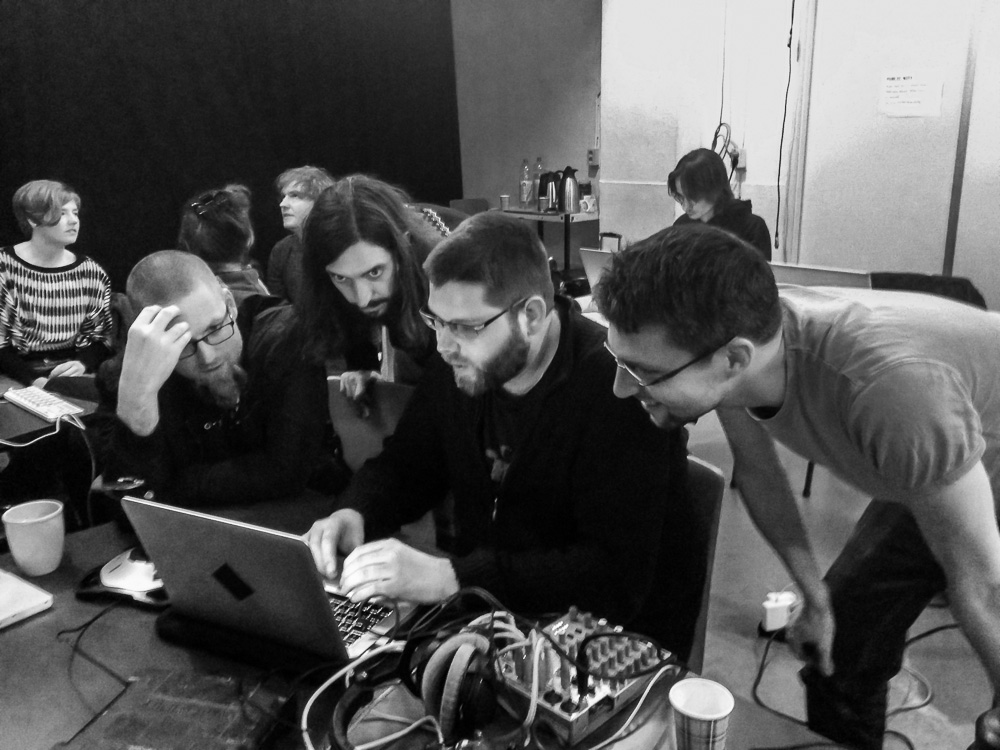
\includegraphics[width=.9\columnwidth]{../media/20140403-IMG_1667.jpg}
	\caption{Public workshop and open Lab at STEIM}
	\label{fig:media_20140403-IMG_1667}
\end{figure}



\section{Implementation}
\label{sec:implementation}


ImmLib is implemented as a set of classes for the SuperCollider language \cite{mccartney2002-ret}. The control elements of devices are accessed through the |MKtl| class. A control element is a part of a controller that generates a one-dimensional stream of events, accepts a one-dimensional stream of events or both of the above. Each MKtl object has elements such as sliders or knobs. It is possible to assign an action to such an element that is evaluated every time the value of that element gets updated. Elements are instances of MKtlElement and are kept in a tree-like data structure using nested arrays and dictionaries which represents the spatial grouping of control elements in the physical controller. The elements can also be accessed from a flat array using the |allElement| method. The |elementDescription| variable of MKtlElement contains a dictionary with information about that element such as it's type (a button, a slider, etc.) and control spec for scaling incoming values. This dictionary can be used to extract multiple elements from the data structure by filtering using a conditional expression, for instance retrieving all elements of type |slider|.

Each MKtl has a name, and only one MKtl is active with same name at any given time. MKtl's can be retrieved from a global dictionary by name, using the |MKtl('name')| syntax. The system keeps a global set of auto-generated names for all the controllers that have description files. These short names are auto-generated from the name of the device plus a number starting from zero indexing multiple identical devices (e.g. |'nnkn0'| from |'nanoKONTROL'|). If a user tries to fetch an MKtl with one of the auto-generated names and it is not yet created the system will look for the corresponding device and if it is found an MKtl is created from the description file and connected to the device by creating MIDI or HID responders. This feature means the user can initialize an MKtl for a given device using always the same single line of code.

\begin{Verbatim}
k = MKtl('nnkn20');
\end{Verbatim}

Actions are added to elements by setting the MKtlElements' |action| to a function. This function is called every time an event is received from that control and it is passed the MKtlElement instance. It's possible to add and remove multiple actions to the same element using the |addAction| and |removeAction| methods which use the |FunctionList| class.

\begin{Verbatim}
//add action
MKtl('nnkn20')
.elements[\sl][0]
.action = { |e|
  var freq = e.value
  .linlin(0.0,1.0,300,3000);
  x.set(\freq, freq)
};

//remove action
MKtl('nnkn20')
.elements[\sl][0]
.action = nil
\end{Verbatim}

Some elements (with |ioType| |'out'| or |'inout'|) can also send values back to the device, this is done using the |value_| method of |MKtlElement|.

\begin{Verbatim}	
MKtl('bcr20000')
.elements[\kn][0][0]
.value_(0.3)
\end{Verbatim}

\subsection{Unifications of interface implementations}
\label{sub:unifications_of_interface_implementations}

The Modality toolkit works uniformly across multiple protocols. The base class MKtl provides the generic functionality and the children classes (|HIDMKtl|, |MIDIMktl|, |OSCMKtl|, etc.) implement the specific back-end for each protocol. Since the interface for using Modality is defined in |MKtl| and |MKtlElement|, which are protocol agnostic, the syntax and semantics remain uniform across all protocols. The incoming values of from the device are also scaled to be in the range $[0,1]$ and outgoing values are expected to be in $[0,1]$ range and then scaled to the range used by the specific protocol. This facilitates switching between devices that use different protocols while keeping the event logic unaltered.

\subsection{Description files}
\label{sub:descriptions_files}

In order for Modality to be able to use a device a \textit{device description} file must be available for it.  A device description file characterizes and labels each element and provides the shape of the data structure used to access elements. It is implemented using one text file per device containing an sclang dictionary with (at least) fields |protocol| (only one protocol allowed per device, currently only HID and MIDI implemented), |device| (the operating system provided name of the device) and |description|. The 'description' field contains a dictionary with a tree-like structure, where the value at each key can be another dictionary or array and where the leafs contain a dictionary describing each element. These element dictionaries contain the technical specifications of the element, namely identification information (e.g. for MIDI, the MIDI number and channel), the physical type of control (button, slider, etc.) and a \textit{ControlSpec} that specifies how to convert the incoming values to the range $[0,1]$.   \emph{Slould we include the ABNF definition  in an annex ? point to it online ?} Following is the element dictionary for a button of a MIDI device.

\begin{Verbatim}
\rew: (
	\midiMsgType: \cc,
	\type: \button,
	\midiChan: 0,
	\midiNum: 47,
	\spec: \midiBut,
	\mode: \push
)
\end{Verbatim}

Elements which are physically (or virtually) grouped on the device such as with pages, rows or columns are grouped together in the description file using arrays. For instance the third button on the second row of page 4 of a Korg NanoKONTROL can be accessed with the following code:

\begin{Verbatim}
MKtl('nnkn0').elements[\sl][3][1][2]
\end{Verbatim}

The hierarchical grouping of elements also facilitates bulk addressing of elements by traversing the hierarchy starting at the desired node. For instance, it's easy to programatically add actions to multiple elements:

\begin{Verbatim}
MKtl('nnkn0').elements[\sl]
.do{ |xs, page|
 xs.do{ |xs, row|
  xs.do{ |element, column|
   element.action = 
    {[page, row, column].postln}
  }
 }
}
  		
\end{Verbatim}

The standard order for grouped elements is first page, then row starting from the top of controller and finally column starting from the left of the controller.

New devices can be added to modality easily, all that is needed is to write the corresponding device description file. If a user tries to access a device for which there is still no description file available the toolkit can help the user with the creation of the description file. For HID devices a description file can be generated using the |HIDExplorer| class from the information provided by the HID stack at the operating system level. For MIDI devices the user is asked to press or move all the physical controls available and then a description file is generated with the recorded data. In both cases the user should then supply suitable labels or placement in an array for each element, and complete or correct the information provided.





\section{Islands and Bridges, uniform protocols}
\label{sec:islands_and_bridges_uniform_protocols}


\begin{itemize}
	\item Modality toolkit + Various Mixed Things + closely related
	\item more related libs - FP/FRP, wslib, JITLibExtensions, 
		all of Marijes device related quarks, etc 
\end{itemize}

\subsection{ Uniform devices (MIDI, HID, OSC, GUI, Serial) }

		with rich descriptions, hierarchical names for all elements
		FakeGUI for everything


\subsection{ Uniform destinations}

		set messages, RelSet, SoftSet, // if Influx, influence

\emph{ miguel: I'm a bit skeptical about us really having a uniform protocol for destinations. MKtl allows registering call-backs for actions, so does Influx, etc, ok, but so do the stock SC guis, MIDIFunc, etc.  I wonder if we are not claiming too much by saying we have created uniform protocols when all that we are doing is providing call-backs which are known and used everywhere in SuperCollider. One could argue all of Supercollider uses a uniform protocol which is calling methods on objects. Maybe I'm missing something here.
}
 
		
\begin{figure}[h]
	\centering
		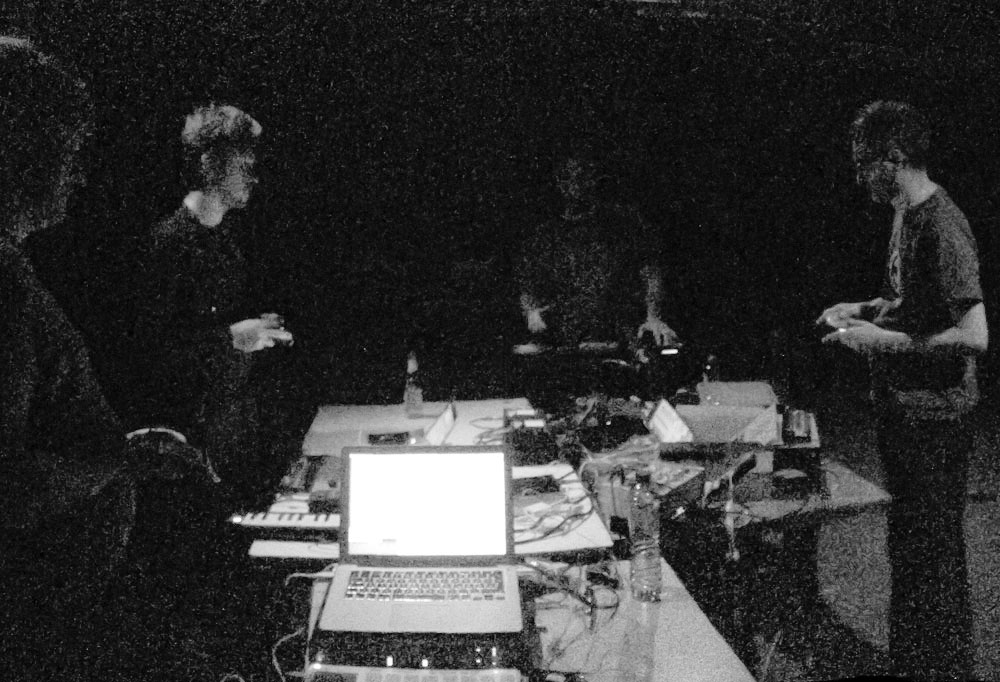
\includegraphics[width=.9\columnwidth]{../media/20140405-IMG_1691.jpg}
	\caption{Modality Concert 2014 at OT301}
	\label{fig:media_20140405-IMG_1691}
\end{figure}

\subsection{Transformer islands} 

What are they supposed to be ? Why are there several different ones ?	
	
\subsubsection{MDispatch}	

describe : An initial attempt, interesting but didn't catch on.
		
\subsubsection{FRP}

An electronic instrument can be though of as set of inputs from control devices, a set of audio units or processes that create audio units and control logic to allow incoming events from the physical devices to affect the state of the audio units. 

The traditional method of dealing with incoming events is through call-back functions. A call-back function is registered and it is called every time an event is received. Call-back functions, although easy to define lack composability and require all the basic patching to be handled by user. Functional Reactive Programming, or FRP, is a paradigm for programming dynamic and reactive systems using first-class composable abstractions that tries to address some of these issues. The two main abstractions are event streams (sequences of discrete-time event occurrences) and behaviours or signals (time-varying values). FRP is a novel programing technique still being actively researched, nevertheless there are already some practical applications of it, mostly for web development (Flapjax, ELM, reactive-web). Most of the original work on FRP was done on the Haskell programming language\footnote{Haskell is a modern, pure, statically typed functional programming language.} with two main flavors, Classic FRP\cite{elliott_functional_1997,elliott_push-pull_2009} and Arrowized FRP~\cite{hudak_arrows_2003}.

The FRP paradigm seemed promising for the construction of musical digital instruments, so in order to make it available in the SuperCollider language the \emph{reactive-web} library from the Scala language was ported to SuperCollider and extended. Ideas from \emph{reactive-banana}, a modern FRP library for Haskell, were also incorporated. This SuperCollider FRP implementation is part of the FPLib library~\cite{-fpl} which makes available a number of functional programming constructs in SuperCollider such as Monads, Applicative, Functors and Monoids.
 
In FP-Lib the main entities for FRP are the EventStream and FPSignal classes. Signals are slightly different from the behaviors of Classic FRP: behaviors model any continuous time function $f:Time\rightarrow A$, while signals only model step functions.  Outputs are defined in terms of inputs using \emph{combinators} (pure functions) applied to the signals or event streams which form an \emph{event graph}. To get events into the event graph the system has to register with external sources, the inputs, and to have any effect on the outside world it must perform actions based on the outputs of the event graph. The \emph{event graph} together with \emph{inputs} and \emph{outputs} forms an\emph{event network}. To build an \emph{event network} the inputs, outputs and event graph are described in a definition which can then be compiled into a working event network. The compiled event network can be started and stopped at any moment, stopping it disconnects from all registered event sources and stops performing output actions. The connecting and disconnecting from objects outside of the event network is atomic. 

It's possible to create complex programs with time-dependent logic by composing  event streams and signal. Below we list some of the basic operations available:

\begin{itemize}

\item transforming event streams into signals and vice-versa:
\begin{Verbatim}
sig1 = es1.hold(0.0)
es2 = sig2.changes
\end{Verbatim}
\item Merging n event streams into one event stream by taking events from any of the incoming streams:
\begin{Verbatim}
mergedEs = es1 | es2 | es3 | es4
\end{Verbatim}
\item Filtering events of an event stream using a function that returns a boolean:
\begin{Verbatim}
es.filter({ |x| x > 0.5 })
\end{Verbatim}
\item Keeping state that can be influenced by several different event streams by  associating each event stream with a state altering function. The state if first set to an initial value, then each time the event streams receive an event it generates a new function to be applied to the current value of the state. For example, a counter that can be incremented by one event stream and decremented with another:
\begin{Verbatim}
(es1.collect(_+1)|es2.collect(_-1))
.injectF(0) 
\end{Verbatim}
\item Merging n signals using an n-ary function. This is possible to do with signals but not with event streams, since only signals remember their last value. For example, converting two signals carrying x and y coordinates to one signal carrying the angle: 
\begin{Verbatim}
atah2(_,_).lift.(xSig, ySig)
\end{Verbatim}
\item Applying a time-varying function (stored in an signal) to an event stream. This allows event streams to use previous values from other nodes in the graph. For example, starting a synth on pressing a pad with frequency determined by the last value of a slider:
\begin{Verbatim}
{ |f,onoff| IO{ Synth(\a,[\freq,f]) } }
<\$> sliderSig <@> padEs 
\end{Verbatim}
\item Dynamic event switching: changing the event graph by running a function on an incoming event that returns the new event stream or signal to use. For example, every time a signal emits an int $n$, create a new signal that merges the first $n$ elements of a list of signals using an averaging function: 
\begin{Verbatim}
sig1.switchInto{ |n|
  listOfSignals[..n].sequence
  .collect{ |xs| xs.sum / xs.size }
}
\end{Verbatim}
All FRP objects created inside the function are automatically disposed off when the function is run again preventing leaks.
\end{itemize}

In the FP-Lib, inputs to the event graph can come from MIDI or HID (via the
Modality Toolkit), OSC, GUIs or Timers and are declared using  the |enIn| method (signal) or |enInES| (event stream) method. Outputs are declared by calling |enOut| on a signal or event stream that carries actions to be performed (elements of the IO monad, which in SuperCollider are essentially just functions). For convenience there are predefined actions available called \textit{sinks}. Passing an FRP object to a sink will execute the default action of the sink using the values emitted by the object.

FPLib can be used in conjunction with UnitLib, in which case the definition of the event network should return a dictionary of synth control names to Signals or event streams. The output of the frp objects can then be automatically scaled to the range of the parameter of the synth, since the unit keeps a control spec for each control in the SynthDef.

The code used to create an event graph for an instrument is highly reusable since any parts of the graph can be repackaged into a single function and used elsewhere. Since all the functions used to construct the graph are pure\footnote{SuperCollider is not a typed pure FP language like Haskell, so there are no guarantees that the functions passed by the user to the to the FRP combinators are actually pure, it's up to the user to make sure that this is the case.} it's possible to abstract a subset of them into a single function and be confident that the result will be identical. This makes it easy to build a personal library of event logic functions that can be re-used for different instruments or different parts of the same instrument.

Several use cases put forward by the Modality Team have been implemented using FPLib and so far the system as shown itself capable of creating complex event graphs used in digital instruments.

\subsubsection{Influx}

describe

\subsubsection{others}

which ones ?

\section{Examples / Use Cases}
\label{sec:examples_use_cases}


\subsection{MPD 18}
\label{sub:mpd_18}

The MPD18 has 16 Buttons and a slider.

\begin{description}
 \item [Sound Buttons] Buttons 1-3 are mapped to adsr enveloped sound sources.
        By pushing them down sound turns on; releasing: sound off.
    the Slider sets amplitude (or pitch) for the (sound)source of the currently depressed button.
 \item [Memory Slots] Buttons 5-16 represent 'memory' positions (initially not mapped)
        if sound is assigned (see below), sound is played when button depressed.
 \item [Shift Button] Button 4 is a 'shift key'. When depressed
        Sound Buttons don't trigger any sound but select the active slot. This can be followed by
        depressing a Memory Slot button, which assigns the selected sound to that pad.
        if you release the shift key before assignment, nothing happens.
        assigning a copy to an already assigned memory slot replaces existing
        mute copy +[Sound Button then Shift button]
        Sound Button triggers sound
        depress Memory Slot button, assigning the sound to the pad, with sound
\end{description}
       
\subsection{Switching actions}
\label{sub:switching_actions}

Switching actions from one controller to another mid-way through a performance.

\subsection{An example of a performance setup with influx and KtlLoop}

\emph{Would this make sense here ?}

\section{Conclusions}
\label{sec:conclusions}



Claims to originality:
* incoming data is associated with a rich knowledge of what generated it. possible to query elements based on type.
* access to elements done in a logical and memorize-able way, both through the auto-generated device names and element hierarchy.
* automatic initialization reduces startup to one line of code.
* Uniform access to controls from devices across multiple controllers and protocols.
* Several ways to take inputs and create complex instruments investigated.

We have showed beyond doubt that Modality is the best thing since sliced bread. It surpasses all other solutions out there both already invented and to be invented in the future. Resistance is futile, you will modalidated.


\begin{acknowledgments}
The Modality team is (in alphabetical order):
    Marije Baalman,
    Tim Blechmann,
    Till Bovermann,
    Alberto de Campo,
    Jeff Carey,
    Bj\o{}rnar Habbestad,
    Dominik Hildebrand Marques Lopes,
    Amelie Hinrichsen,
    Robert van Heumen,
    Hannes Hoelzl,
    Miguel Negr\~{a}o, and
    Wouter Snoei.
Associated organisations are (in alphabetical order):
BEK,
the project \emph{Design, Development and Dissemination of New Musical Instruments} of UdK Berlin/TU Berlin, supported by the Einstein Foundation,
nescivi, and
STEIM.

The Modality meetings have been funded by Bergen Kommune, Nordisk Kulturfond and Creative Industries Fund NL.


\end{acknowledgments} 

%%%%%%%%%%%%%%%%%%%%%%%%%%%%%%%%%%%%%%%%%%%%%%%%%%%%%%%%%%%%%%%%%%%%%%%%%%%%%
%bibliography here
\bibliography{icmcmodality}

\end{document}
